%\title{RGPV Thesis Abhushan}
\RequirePackage[l2tabu]{nag}		% Warns for incorrect (obsolete) LaTeX usage
%
%
% File: memoirthesis.tex
% Author: Abhushan Sahu
% Description: Contains the thesis template using memoir class,
% which is mainly based on book class but permits better control of 
% chapter styles for example. This template is an adaptation and 
% modification of Oscar's.
% 
% Memoir is a flexible class for typesetting poetry, fiction, 
% non-fiction and mathematical works as books, reports, articles or
% manuscripts. CTAN repository is found at:
% http://www.ctan.org/tex-archive/macros/latex/contrib/memoir/
%
%
% UoB guidelines for thesis presentation were found at:
% http://www.bris.ac.uk/esu/pg/pgrcop11-12topic.pdf#page=49
%
% UoB guidelines:
%
% The dissertation must be printed on A4 white paper. Paper up to A3 may be used
% for maps, plans, diagrams and illustrative material. Pages (apart from the
% preliminary pages) should normally be double-sided.
%
% Memoir class loads useful packages by default (see manual).
\documentclass[a4paper,11pt,leqno,openbib]{memoir} %add 'draft' to turn draft option on (see below)
%
%
% Adding metadata:
\usepackage{datetime}
\usepackage{ifpdf}
\ifpdf
\pdfinfo{
   /Author (Author's name)
   /Title (Bachelor Thesis)
   /Keywords (One; Two;Three)
   /CreationDate (D:\pdfdate)
}
\fi
% When draft option is on. 
\ifdraftdoc 
	\usepackage{draftwatermark}				%Sets watermarks up.
	\SetWatermarkScale{0.3}
	\SetWatermarkText{\bf Draft: \today}
\fi
%
% Declare figure/table as a subfloat.
\newsubfloat{figure}
\newsubfloat{table}
% Better page layout for A4 paper, see memoir manual.
\settrimmedsize{297mm}{210mm}{*}
\setlength{\trimtop}{0pt} 
\setlength{\trimedge}{\stockwidth} 
\addtolength{\trimedge}{-\paperwidth} 
\settypeblocksize{634pt}{448.13pt}{*} 
\setulmargins{4cm}{*}{*} 
\setlrmargins{*}{*}{1.5} 
\setmarginnotes{17pt}{51pt}{\onelineskip} 
\setheadfoot{\onelineskip}{2\onelineskip} 
\setheaderspaces{*}{2\onelineskip}{*} 
\checkandfixthelayout
%
\frenchspacing
% Font with math support: New Century Schoolbook
\usepackage{fouriernc}
\usepackage[T1]{fontenc}
%
% UoB guidelines:
%
% Text should be in double or 1.5 line spacing, and font size should be
% chosen to ensure clarity and legibility for the main text and for any
% quotations and footnotes. Margins should allow for eventual hard binding.
%
% Note: This is automatically set by memoir class. Nevertheless \OnehalfSpacing 
% enables double spacing but leaves single spaced for captions for instance. 
\OnehalfSpacing 
%
% Sets numbering division level
\setsecnumdepth{subsection} 
\maxsecnumdepth{subsubsection}
%
% Chapter style (taken and slightly modified from Lars Madsen Memoir Chapter 
% Styles document
\usepackage{calc,soul,fourier}
\makeatletter 
\newlength\dlf@normtxtw 
\setlength\dlf@normtxtw{\textwidth} 
\newsavebox{\feline@chapter} 
\newcommand\feline@chapter@marker[1][4cm]{%
	\sbox\feline@chapter{% 
		\resizebox{!}{#1}{\fboxsep=1pt%
			\colorbox{gray}{\color{white}\thechapter}% 
		}}%
		\rotatebox{90}{% 
			\resizebox{%
				\heightof{\usebox{\feline@chapter}}+\depthof{\usebox{\feline@chapter}}}% 
			{!}{\scshape\so\@chapapp}}\quad%
		\raisebox{\depthof{\usebox{\feline@chapter}}}{\usebox{\feline@chapter}}%
} 
\newcommand\feline@chm[1][4cm]{%
	\sbox\feline@chapter{\feline@chapter@marker[#1]}% 
	\makebox[0pt][c]{% aka \rlap
		\makebox[1cm][r]{\usebox\feline@chapter}%
	}}
\makechapterstyle{daleifmodif}{
	\renewcommand\chapnamefont{\normalfont\Large\scshape\raggedleft\so} 
	\renewcommand\chaptitlefont{\normalfont\Large\bfseries\scshape} 
	\renewcommand\chapternamenum{} \renewcommand\printchaptername{} 
	\renewcommand\printchapternum{\null\hfill\feline@chm[2.5cm]\par} 
	\renewcommand\afterchapternum{\par\vskip\midchapskip} 
	\renewcommand\printchaptertitle[1]{\color{gray}\chaptitlefont\raggedleft ##1\par}
} 
\makeatother 
\chapterstyle{daleifmodif}
%
% UoB guidelines:
%
% The pages should be numbered consecutively at the bottom centre of the
% page.
\makepagestyle{myvf} 
\makeoddfoot{myvf}{}{\thepage}{} 
\makeevenfoot{myvf}{}{\thepage}{} 
\makeheadrule{myvf}{\textwidth}{\normalrulethickness} 
\makeevenhead{myvf}{\small\textsc{\leftmark}}{}{} 
\makeoddhead{myvf}{}{}{\small\textsc{\rightmark}}
\pagestyle{myvf}
%
% Oscar's command (it works):
% Fills blank pages until next odd-numbered page. Used to emulate single-sided
% frontmatter. This will work for title, abstract and declaration. Though the
% contents sections will each start on an odd-numbered page they will
% spill over onto the even-numbered pages if extending beyond one page
% (hopefully, this is ok).
\newcommand{\clearemptydoublepage}{\newpage{\thispagestyle{empty}\cleardoublepage}}
%
%
% Creates indexes for Table of Contents, List of Figures, List of Tables and Index
\makeindex
% \printglossaries below creates a list of abbreviations. \gls and related
% commands are then used throughout the text, so that latex can automatically
% keep track of which abbreviations have already been defined in the text.
%
% The import command enables each chapter tex file to use relative paths when
% accessing supplementary files. For example, to include
% chapters/brewing/images/figure1.png from chapters/brewing/brewing.tex we can
% use
% \includegraphics{images/figure1}
% instead of
% \includegraphics{chapters/brewing/images/figure1}
\usepackage{import}

% Add other packages needed for chapters here. For example:
\usepackage{lipsum}					%Needed to create dummy text
\usepackage{amsfonts} 					%Calls Amer. Math. Soc. (AMS) fonts
\usepackage[centertags]{amsmath}			%Writes maths centred down
\usepackage{stmaryrd}					%New AMS symbols
\usepackage{amssymb}					%Calls AMS symbols
\usepackage{amsthm}					%Calls AMS theorem environment
\usepackage{newlfont}					%Helpful package for fonts and symbols
\usepackage{layouts}					%Layout diagrams
\usepackage{graphicx}					%Calls figure environment
\usepackage{longtable,rotating}			%Long tab environments including rotation. 
\usepackage[applemac]{inputenc}			%Needed to encode non-english characters 
	\usepackage[section]{placeins}									%directly for mac
\usepackage{colortbl}					%Makes coloured tables
\usepackage{wasysym}					%More math symbols
\usepackage{mathrsfs}					%Even more math symbols
					%Helps to place figures, tables, etc. 
\usepackage{verbatim}					%Permits pre-formated text insertion
\usepackage{upgreek }					%Calls other kind of greek alphabet
\usepackage{latexsym}					%Extra symbols
\usepackage[square,numbers,
		     sort&compress]{natbib}		%Calls bibliography commands 
\usepackage{url}						%Supports url commands
\usepackage{etex}						%eTeXÕs extended support for counters
\usepackage{fixltx2e}					%Eliminates some in felicities of the 
									%original LaTeX kernel
\usepackage[spanish,english]{babel}		%For languages characters and hyphenation
\usepackage{color}                    				%Creates coloured text and background
\usepackage[colorlinks=true,
		     allcolors=black]{hyperref}              %Creates hyperlinks in cross references
\usepackage{memhfixc}					%Must be used on memoir document 
									%class after hyperref
\usepackage{enumerate}					%For enumeration counter
\usepackage{footnote}					%For footnotes
\usepackage{microtype}					%Makes pdf look better.
\usepackage{rotfloat}					%For rotating and float environments as tables, 
									%figures, etc. 
\usepackage{alltt}						%LaTeX commands are not disabled in 

\usepackage{floatpag}             %verbatim-like environment
\usepackage[version=0.96]{pgf}			%PGF/TikZ is a tandem of languages for producing vector graphics from a 
\usepackage{tikz}						%geometric/algebraic description.
\usepackage{pdfpages}
\usetikzlibrary{arrows,shapes,snakes,
		       automata,backgrounds,
		       petri,topaths}				%To use diverse features from tikz		
%							
%Reduce widows  (the last line of a paragraph at the start of a page) and orphans 
% (the first line of paragraph at the end of a page)
\widowpenalty=1000
\clubpenalty=1000
%
% New command definitions for my thesis
%
\newcommand{\keywords}[1]{\par\noindent{\small{\bf Keywords:} #1}} %Defines keywords small section
\newcommand{\parcial}[2]{\frac{\partial#1}{\partial#2}}                             %Defines a partial operator
\newcommand{\vectorr}[1]{\mathbf{#1}}                                                        %Defines a bold vector
\newcommand{\vecol}[2]{\left(                                                                         %Defines a column vector
	\begin{array}{c} 
		\displaystyle#1 \\
		\displaystyle#2
	\end{array}\right)}
\newcommand{\mados}[4]{\left(                                                                       %Defines a 2x2 matrix
	\begin{array}{cc}
		\displaystyle#1 &\displaystyle #2 \\
		\displaystyle#3 & \displaystyle#4
	\end{array}\right)}
\newcommand{\pgftextcircled}[1]{                                                                    %Defines encircled text
    \setbox0=\hbox{#1}%
    \dimen0\wd0%
    \divide\dimen0 by 2%
    \begin{tikzpicture}[baseline=(a.base)]%
        \useasboundingbox (-\the\dimen0,0pt) rectangle (\the\dimen0,1pt);
        \node[circle,draw,outer sep=0pt,inner sep=0.1ex] (a) {#1};
    \end{tikzpicture}
}
\newcommand{\range}[1]{\textnormal{range }#1}                                             %Defines range operator
\newcommand{\innerp}[2]{\left\langle#1,#2\right\rangle}                                 %Defines inner product
\newcommand{\prom}[1]{\left\langle#1\right\rangle}                                         %Defines average operator
\newcommand{\tra}[1]{\textnormal{tra} \: #1}                                                       %Defines trace operator
\newcommand{\sign}[1]{\textnormal{sign\,}#1}                                                   %Defines sign operator
\newcommand{\sech}[1]{\textnormal{sech} #1}                                                  %Defines sech
\newcommand{\diag}[1]{\textnormal{diag} #1}                                                    %Defines diag operator
\newcommand{\arcsech}[1]{\textnormal{arcsech} #1}                                       %Defines arcsech
\newcommand{\arctanh}[1]{\textnormal{arctanh} #1}                                         %Defines arctanh
%Change tombstone symbol
\newcommand{\blackged}{\hfill$\blacksquare$}
\newcommand{\whiteged}{\hfill$\square$}
\newcounter{proofcount}
\renewenvironment{proof}[1][\proofname.]{\par
 \ifnum \theproofcount>0 \pushQED{\whiteged} \else \pushQED{\blackged} \fi%
 \refstepcounter{proofcount}
 \normalfont 
 \trivlist
 \item[\hskip\labelsep
       \itshape
   {\bf\em #1}]\ignorespaces
}{%
 \addtocounter{proofcount}{-1}
 \popQED\endtrivlist
}
%
%
% New definition of square root:
% it renames \sqrt as \oldsqrt
\let\oldsqrt\sqrt
% it defines the new \sqrt in terms of the old one
\def\sqrt{\mathpalette\DHLhksqrt}
\def\DHLhksqrt#1#2{%
\setbox0=\hbox{$#1\oldsqrt{#2\,}$}\dimen0=\ht0
\advance\dimen0-0.2\ht0
\setbox2=\hbox{\vrule height\ht0 depth -\dimen0}%
{\box0\lower0.4pt\box2}}
%
% My caption style
\newcommand{\mycaption}[2][\@empty]{
	\captionnamefont{\scshape} 
	\changecaptionwidth
	\captionwidth{0.9\linewidth}
	\captiondelim{.\:} 
	\indentcaption{0.75cm}
	\captionstyle[\centering]{}
	\setlength{\belowcaptionskip}{10pt}
	\ifx \@empty#1 \caption{#2}\else \caption[#1]{#2}
}
%
% My subcaption style
\newcommand{\mysubcaption}[2][\@empty]{
	\subcaptionsize{\small}
	\hangsubcaption
	\subcaptionlabelfont{\rmfamily}
	\sidecapstyle{\raggedright}
	\setlength{\belowcaptionskip}{10pt}
	\ifx \@empty#1 \subcaption{#2}\else \subcaption[#1]{#2}
}
%
%An initial of the very first character of the content
\usepackage{lettrine}
\newcommand{\initial}[1]{%
	\lettrine[lines=3,lhang=0.33,nindent=0em]{
		\color{gray}
     		{\textsc{#1}}}{}}
%
% Theorem styles used in my thesis
%
\theoremstyle{plain}
\newtheorem{theo}{Theorem}[chapter]
\theoremstyle{plain}
\newtheorem{prop}{Proposition}[chapter]
\theoremstyle{plain}
\theoremstyle{definition}
\newtheorem{dfn}{Definition}[chapter]
\theoremstyle{plain}
\newtheorem{lema}{Lemma}[chapter]
\theoremstyle{plain}
\newtheorem{cor}{Corollary}[chapter]
\theoremstyle{plain}
\newtheorem{resu}{Result}[chapter]
%
% Hyphenation for some words
%
\hyphenation{res-pec-tively}
\hyphenation{mono-ti-ca-lly}
\hyphenation{hypo-the-sis}
\hyphenation{para-me-ters}
\hyphenation{sol-va-bi-li-ty}
%
%
\begin{document}
% UoB guidlines:
%
% Preliminary pages
% 
% The five preliminary pages must be the Title Page, Abstract, Dedication
% and Acknowledgements, Author's Declaration and Table of Contents.
% These should be single-sided.
% 
% Table of contents, list of tables and illustrative material
% 
% The table of contents must list, with page numbers, all chapters,
 % sections and subsections, the list of references, bibliography, list of
% abbreviations and appendices. The list of tables and illustrations
% should follow the table of contents, listing with page numbers the
% tables, photographs, diagrams, etc., in the order in which they appear
% in the text.
% 
\frontmatter
\pagenumbering{roman}
%
%
% File: Title.tex
% Author: Abhushan Sahu
% Description: Contains the title page
%
% UoB guidelines:
% 
% At the top of the title page, within the margins, the dissertation should give the title and, if 
% necessary, sub-title and volume number. If the dissertation is in a language other than English, the 
% title must be given in that language and in English. The full name of the author should be in the 
% centre of the page. At the bottom centre should be the words ?A dissertation submitted to the 
% University of Bristol in accordance with the requirements for award of the degree of ? in the 
% Faculty of ...?, with the name of the school and month and year of submission. The word count of 
% the dissertation (text only) should be entered at the bottom right-hand side of the page.
%
%
\begin{titlingpage}
\begin{SingleSpace}
\calccentering{\unitlength} 
\begin{adjustwidth*}{\unitlength}{-\unitlength}
\vspace*{13mm}
\begin{center}
\rule[0.5ex]{\linewidth}{2pt}\vspace*{-\baselineskip}\vspace*{3.2pt}
\rule[0.5ex]{\linewidth}{1pt}\\[\baselineskip]
{\HUGE A Study in Fall }\\[4mm]
{\Large \textit{Can a tumble save lives?}}\\
\rule[0.5ex]{\linewidth}{1pt}\vspace*{-\baselineskip}\vspace{3.2pt}
\rule[0.5ex]{\linewidth}{2pt}\\
\vspace{6.5mm}
{\large By}\\
\vspace{6.5mm}
{\large\textsc{Abhushan Sahu}}\\
{\large\textsc{Abhinav Singh}}\\
\vspace{11mm}

\includegraphics[scale=0.4]{logos/rgpv_logo}\\
\vspace{6mm}
{\large Department of Information Technology\\
\large Sagar Institute of Research and Technology\\
\vspace{10mm}
\textsc{Rajiv Gandhi Proudyogiki Vishwavidyalaya}}\\
\vspace{11mm}
\textsc{
A dissertation submitted to the Rajiv Gandhi Proudyogiki Vishwavidyalaya in accordance with the requirements of the degree of \textsc{Bachelor of Engineering} in the Faculty of Information Technology.}
\\
\vspace{9mm}
{\large\textsc{MARCH 2015}}
\vspace{12mm}
\end{center}
\begin{flushright}
{\small Word count: 6547}
\end{flushright}
\end{adjustwidth*}
\end{SingleSpace}
\end{titlingpage}
\clearemptydoublepage
%


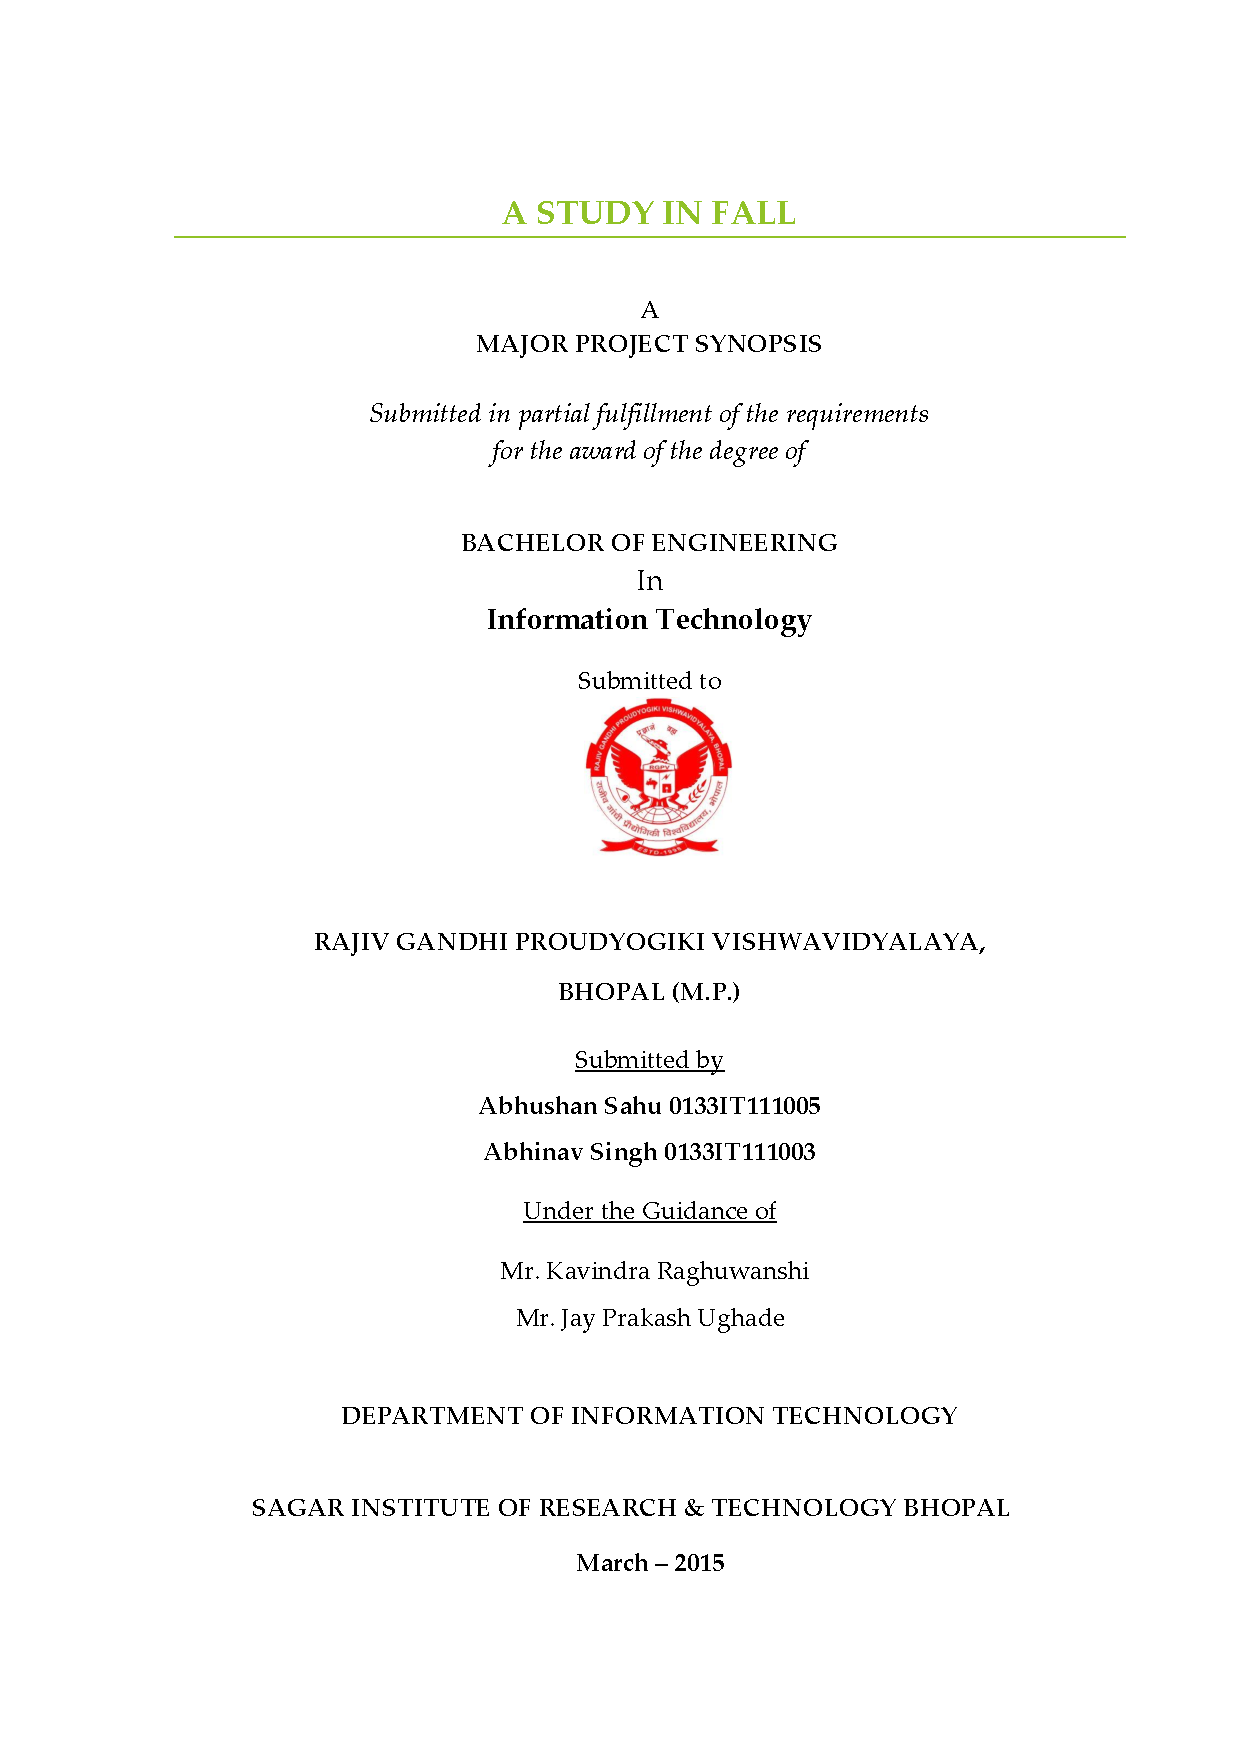
\includepdf[pages={1}]{frontmatter/title2.pdf}
\cleardoublepage
%
%
% File: abstract.tex
% Author: Abhushan Sahu
% Description: Contains the text for thesis abstract
%
% UoB guidelines:
%
% Each copy must include an abstract or summary of the dissertation in not
% more than 300 words, on one side of A4, which should be single-spaced in a
% font size in the range 10 to 12. If the dissertation is in a language other
% than English, an abstract in that language and an abstract in English must
% be included.

\chapter*{Abstract}
\begin{SingleSpace}
\initial{T}he purpose of my project was to model how a certain change in posture of a human body, can be used to determine the ambiance, and thereby working accordingly. Similar tests are used by car manufacturers to signal the airbags to inflate when needed. In testing, subject was regulated to conditions that can result in harm, under laboratory conditions. \\

The research is named under the line, `A Study in Fall', Where the whole study is concentrated during the fall/jerk/accident of the user. The data gathered and assessment that works for is done inside the event. Hence the name, a study `in' fall, rather than `on' or `of'. The research/project has been escorted/guided with the help of two professional doctors. Hence the correctness of the study is in favor of us.\\

I conducted several experiments using myself, and some few volunteers. I further added the knowledge of statistics to determine a pattern in the data. For each experiment, subject has to undergo a fall, or an unexpected anomaly in motion. Further refining of data using R processing, gave a clear window. Detailed study and whole story has been revealed on the inside of the book.\\

The practical implementation aka the project is named, `Helpr'. This is a cell phone application, that works under the climactic part of any accident. Basically the provision of this application work under a very delicate situation when the life of a user hangs in balance, literally. It being a post alarming application activates its procedure after any calamity happens, though it runs always in the background as a service to the phone. With having just a tiny bit of overhead charge for the battery or processing, which is closely negligible.\\

The algorithm is subject to change/update in accordance with future experiments. I initially used the upper bound function, which after a few trials is captured in a window(stated inside). This whole experimentation and real-time data, helps in creation of the application from dust. \\

Further, the structuring and coding part is done under android environment with java as the primary language, this was chosen as it being popular at the time of its creation.


\end{SingleSpace}
\clearpage
\clearemptydoublepage
%
%
% file: dedication.tex
% author: Abhushan Sahu
% description: Contains the text for thesis dedication
%

\chapter*{Dedication and acknowledgements}
\begin{SingleSpace}
\initial{T}his dissertation is dedicated to sole idea of using this intent to make world a better place.\\
  \vspace{5mm} \\
\quad  This project/research was supported/partially supported by anonymous funding, though
\   menial. We thank our colleagues from \textit{Sagar Group of Instituion} who provided insight and expertise that greatly assisted the project/research, although they may not agree with all of the interpretations/conclusions of this paper.
\vspace{10mm} \\
We thank \textit{Dr. Alankar Sahu} for assistance and methodology, and \textit{Dr. Shruti Iyer} for comments that greatly improved the manuscript.
\vspace{10mm} \\
Nevertheless, we express our gratitude toward our families and colleagues for their kind co-operation and encouragement which help us in completion of this project. We are also immensely grateful to their comments on an earlier version of the manuscript, although any errors are our own and should not tarnish the reputations of these esteemed persons.
\end{SingleSpace}
\clearpage
\clearemptydoublepage
%
%
% File: declaration.tex
% Author: Abhushan Sahu
% Description: Contains the declaration page
%
% UoB guidelines:
%
% Author's declaration
%
% I declare that the work in this dissertation was carried out in accordance
% with the requirements of the University's Regulations and Code of Practice
% for Research Degree Programmes and that it has not been submitted for any
% other academic award. Except where indicated by specific reference in the
% text, the work is the candidate's own work. Work done in collaboration with,
% or with the assistance of, others, is indicated as such. Any views expressed
% in the dissertation are those of the author.
%
% SIGNED: .............................................................
% DATE:..........................
%
\chapter*{Author's declaration}
\begin{SingleSpace}
\begin{quote}
\initial{I} declare that the work in this dissertation was carried out in accordance with the requirements of  the University's Regulations and Code of Practice for Degree Programmes and that it  has not been submitted for any other academic award. Except where indicated by specific  reference in the text, the work is the candidate's own work. Work done in collaboration with, or with the assistance of, others, is indicated as such. Any views expressed in the dissertation are those of the author. 
\vspace{5mm} \\
We hereby declare that the Project synopsis entitled ``\emph{A study in fall}'' is our own work, conducted under controlled conditions and obligatory supervision of the guides at Sagar Institute of Research and Technology, Bhopal.
\begin{center}
\vspace{6mm}

\includegraphics[scale=0.25]{logos/sirt_logo}\\
\vspace{6mm}

\end{center}


Any use of the system/code/algorithm/methodology/concept, without the consent of developer should be considered as an intellectual theft or threat to it.
\vspace{2cm} \\
%\noindent
\hspace{-0.75cm}\textsc{SIGNED: .......Abhushan Sahu- 0133IT111005......... DATE: ...................}
\vspace{0.1cm} 
\\

\textsc{SIGNED: .......Abhinav Singh- 0133IT111003......... DATE: ...................}
\end{quote}
\end{SingleSpace}
\clearpage 
\clearemptydoublepage
%
\renewcommand{\contentsname}{Table of Contents}
\maxtocdepth{subsection}
\tableofcontents*
\addtocontents{toc}{\par\nobreak \mbox{}\hfill{\bf Page}\par\nobreak}
\clearemptydoublepage
%
%\listoftables
%\addtocontents{lot}{\par\nobreak\textbf{{\scshape Table} \hfill Page}\par\nobreak}
\clearemptydoublepage
%
\listoffigures
\addtocontents{lof}{\par\nobreak\textbf{{\scshape Figure} \hfill Page}\par\nobreak}
\clearemptydoublepage
%
%
% The bulk of the document is delegated to these chapter files in
% subdirectories.
\mainmatter
%

\import{chapters/chapter01/}{chap01.tex}
\clearemptydoublepage
\import{chapters/chapter01/}{chap02.tex}
\clearemptydoublepage
\import{chapters/chapter01/}{chap03.tex}
\clearemptydoublepage
\import{chapters/chapter01/}{chap04.tex}
\clearemptydoublepage
\import{chapters/chapter01/}{chap05.tex}
\newpage\cleardoublepage

%%
% file: recommendation.tex
% author: Abhushan Sahu
% description: Contains the text for thesis dedication
%

\chapter{Recommendation letter by Institute}
\begin{SingleSpace}
%\initial{T}

\end{SingleSpace}

%
%
% And the appendix goes here

%\appendix
\backmatter
\import{backmatter/}{recommendation.tex}

%
% Apparently the guidelines don't say anything about citations or
% bibliography styles so I guess we can use anything.

\backmatter
\bibliographystyle{siam}
\refstepcounter{chapter}
%\bibliography{thesisbiblio}
\begin{thebibliography}{9}
\bibitem{latexcompanion} 
Donald E. Knuth and Leslie Lamport
\textit{\LaTeX\- Latex}. 
, 1985.

\bibitem{knuthwebsite} 
Knuth: Computers and Typesetting,
\\\texttt{http://www-cs-faculty.stanford.edu/\~{}uno/abcde.html}

\bibitem{newton} 
Sir Isaac Newton. 
\textit{The 
Universal Law of Gravitation}. 
, 1643-1727.

\bibitem{creatively} 
Creatively. 
\textit{https://creately.com/app/}. 


\bibitem{quora} 
Quora. 
\textit{https://www.quora.com/}. 

\bibitem{gov} 
Indian Government data. 
\textit{http://data.gov.in/}. 

\bibitem{tut} 
Bucky's room tutorial. 

\bibitem{stack} 
Stack Overflow. 
\textit{https://stackoverflow.com/}. 

\bibitem{android} 
Android Documentation 
\textit{http://developer.android.com/}. 
, 2008.

\bibitem{acci} 
Personal Accidents
\textit{}. 
, 2010, 2012.

\bibitem{over} 
Overleaf
\textit{https://www.overleaf.com/}. 

\bibitem{map}
Google map API
\textit{https://developers.google.com/maps/}

\end{thebibliography}

%
% Add index
%\printindex
%   
\end{document}